\documentclass[authoryearcitations]{UoYCSproject}

\usepackage{tikz}
\usetikzlibrary{arrows,positioning}

\usepackage{amsmath}

\author{Joshua Asch}

\title{Tracing and Debugging in GP2}

\date{Date TBC}
\supervisor{Detlef Plump}
\MEng
\wordcount{0}


\abstract{
    This is my project!
}


\begin{document}

\maketitle
\listoffigures
\listoftables

\cleardoublepage

\chapter{Introduction}
\label{cha:Introduction}

\section{Introductiony Bit}
\label{sec:IntroductionyBit}

A section introducing the project.

\section{Ethics}
\label{sec:Ethics}

A section discussing the ethics of the project.



\clearpage

\chapter{Literature Review}
\label{cha:LiteratureReview}

%//////////////////////////////////////////////////////////////////////////////

\section{Programming by Graph Transformation}
\label{sec:ProgrammingByGraphTransformation}

%==============================================================================

\subsection{Graph Programming}
\label{sec:GraphProgramming}

Graph programming involves a series of transformations applied to a graph. The
problem being solved must be redefined in terms of a start graph and an algorithm
represented by graph transformations. The final graph at the end of the algorithm
gives the solution to the problem.

Historically, programming by graph transformation required using a programming
language such as C or Java, implementing data structures to represent graphs, and
directly making modifications to the graph in the program. However, recently some
attempts have been made to create tools for graph programming which abstract away
the representation of the graphs, allowing the programmer to focus on the program itself.

Some of these tools include PROGRES \citep{schurr1999}, AGG \citep{ermel1999},
GROOVE \citep{rensink2004}, and, most recently, GP2 \citep{bak2015}. All of these
are domain-specific languages for graph programming which also provide a graphical
interface to describe graphs and transformations.

These kinds of tools take a representation of a graph program, as defined in their
graphical editor, and transform this into a runnable program. This can be implemented
in Java (in the case of AGG and GROOVE) or in C (in the case of PROGRES and GP2). This
program can then be executed to find the output graph generated by the algorithm.

%==============================================================================

\subsection{The GP2 Language}
\label{sec:TheGP2Language}

GP2 is a programming language developed at the University of York \citep{bak2015},
an updated implementation of the original language, GP \citep{plump2009}. It is
designed for writing programs at a high level, to perform graph transformations 
without having to implement data structures to represent the graphs in more
traditional lower level languages such as C.

Programming in GP2 consists of an input graph, known as the \emph{host graph}, a
set of \emph{rules}, and a \emph{program} which defines the order in which to
apply the rules. Running a GP2 program on a host graph produces a new graph as
a result, called the \emph{output graph}.

\subsubsection{Rules}
\label{sec:Rules}

Rules are the basic building blocks of a GP2 program and are defined by a
left-hand-side (LHS), a right-hand-side (RHS), and optionally a conditional
clause. A rule can be thought of as the definition of a transformation; a subgraph
matching the LHS of the rule is transformed to resemble the RHS. An example of a
GP2 rule is shown in \autoref{fig:RuleInGP2}.

\begin{figure}
    \begin{center}
        \begin{tabular}{l}

            \texttt{link}

            \\\\

            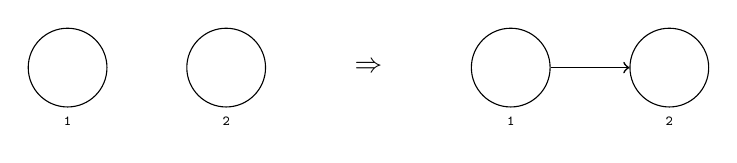
\begin{tikzpicture}
                [vertex/.style={circle,draw,minimum size=10mm},
                 post/.style={<-,semithick}]

                \node         (transition) {$\Rightarrow$}                                {};

                \node[vertex] (lhs 2) [label=below:\tiny{\texttt{2}},left=of transition]  {};
                \node[vertex] (lhs 1) [label=below:\tiny{\texttt{1}},left=of lhs 2]       {};

                \node[vertex] (rhs 1) [label=below:\tiny{\texttt{1}},right=of transition] {};
                \node[vertex] (rhs 2) [label=below:\tiny{\texttt{2}},right=of rhs 1]      {}
                    edge[post] (rhs 1);

            \end{tikzpicture}

            \\

            \texttt{where not edge(1, 2)}

        \end{tabular}
    \end{center}
    \caption{A rule in GP2}
    \label{fig:RuleInGP2}
\end{figure}

The conditional clause is used to specify additional constraints on the subgraph
matching the LHS. Any match has to both match the LHS and conform to the constraints
defined by the conditional clause.

In a compiled program, a rule is split into two phases. The \emph{match} phase
searches the current graph for a subgraph which matches the LHS of the rule. If
a match is found, the program moves on to the second phase, the \emph{application}.
To ensure consistent output between successive program executions, rule matches are
chosen deterministically by the compiled program. If no match is found for the LHS,
the rule is considered \emph{failed}.

During the application phase, any nodes and edges present in the LHS but not the RHS
will be deleted, and any nodes and edges present in the RHS but not the LHS will be
created. At the end of the application phase, the subgraph will match the RHS of the
rule definition. The new graph created by the application of this rule, an \emph{intermediate
graph}, is then used as the input to the next part of the program.

In the example in \autoref{fig:RuleInGP2}, the program will search for a subgraph
containing two nodes without an edge connecting them. If a match is found, it will
be transformed to resemble the RHS by adding an edge between the nodes.

\subsubsection{Programs}

A GP2 program defines the order in which to apply rules using 8 simple control
structures:

\begin{description}
    \item[\textsc{Sequence}]
    Two subprograms separated by a semicolon ``\texttt{P; Q}'' are applied
    one after the other.

    \item[\textsc{Rule Set}]
    Subprograms in curly braces ``\texttt{\{P, Q, R\}}'' define a set, where
    exactly one subprogram from the set is executed, unless no subprograms in
    the set can be matched. The subprogram to execute is chosen deterministically.

    \item[\textsc{If-Then-Else}]
    In the statement ``\texttt{if C then P else Q}'', the sub-program \texttt{C}
    is executed, and the result, i.e. success or failure, is recorded, before
    reverting any changes caused by C. Then, if C succeeded, \texttt{P} is
    executed on the original graph. If it failed, then \texttt{Q} is executed on
    the original graph. Note that by taking a copy first, any changes made by
    \texttt{C} are reverted before executing either \texttt{P} or \texttt{Q}.

    \item[\textsc{Try-Then-Else}]
    Similar to \textsc{If-Then-Else}, but \texttt{C} is only reverted if it fails.
    Thus any changes made by \texttt{C} are \emph{not} reverted before executing
    \texttt{P}, but they \emph{are} reverted before executing \texttt{Q}.

    \item[\textsc{As-Long-As-Possible}]
    A subprogram followed by an exclamation point ``\texttt{P!}'' is matched and
    applied repeatedly until it cannot be matched any more. The final attempt to
    match the LHS will \emph{not} consider the rule \emph{failed}.

    \item[\textsc{Procedure}]
    Similar to a C preprocessor macro, a procedure is simply a named subprogram
    where any reference to the procedure name can be replaced with the definition
    of the procedure.

    \item[\textsc{Skip}]
    A no-op which always succeeds, and does not affect the graph. Invoked using the
    keyword ``\texttt{skip}''.

    \item[\textsc{Fail}]
    A no-op which always fails and does not affect the graph. This is the same as
    attempting to execute a rule for which there are no matches. Invoked using
    the keyword ``\texttt{fail}''.
\end{description}

For GP2, a subprogram is either a single rule, referenced by its name, or one of
the above control structures. Therefore it is possible to nest control structures
to create more complex programs.

In general, execution of a program continues until either all statements are
executed, or until a statement results in an attempt to apply a rule which has
no matches in the graph. The exceptions to this are \textsc{As-Long-As-Possible}
statements, and the conditional statements in \textsc{If-Then-Else} and
\textsc{Try-Then-Else} structures. In these cases, a failure to match a rule
does not halt execution of the program.

\autoref{fig:ExampleProgramDefinition} shows an example GP2 program, the same
program used as a case study in Bak's original thesis on GP2
\citep[pp.126]{bak2015}. It is a simple program which determines whether a graph
is \emph{2-colourable}, that is, its nodes can be coloured using two different
colours without two nodes of the same colour being connected by an edge.

This program consists of four rules and uses many of the constructs outlined
previously, including \textsc{Try-Then-Else}, \textsc{If-Then-Else},
\textsc{Rule Set}s, \textsc{As-Long-As-Possible} and \textsc{Procedure}s.

\begin{figure}
    \begin{center}
        \emph{An example of a program will go here...}
    \end{center}
    \caption{Definition of 2-colouring in GP2}
    \label{fig:ExampleProgramDefinition}
\end{figure}

\begin{figure}
    \begin{center}
        \emph{An execution of 2-colouring will go here...}
    \end{center}
    \caption{Example execution of 2-colouring}
    \label{fig:ExampleProgramExecution}
\end{figure}

An example execution of the 2-colouring program is shown in \autoref{fig:ExampleProgramExecution}.
Starting with an uncoloured graph, the algorithm picks a node and colours it red
using the \texttt{init} rule. It then traverses the graph colouring nodes in
alternating colours using the \texttt{colour\_blue} and \texttt{colour\_red} rules,
by defining them as a \textsc{Rule Set} in a \textsc{Procedure} and executing
it \textsc{As-Long-As-Possible}. When no more uncoloured nodes are present in the
graph, the \texttt{Colour} procedure will be unable to match any further rules,
so it will end.

To check whether the produced colouring is valid, the entire \texttt{Main}
procedure is wrapped in a \textsc{Try-Then-Else} statement. After executing
\texttt{Colour}, the \texttt{Invalid} procedure runs. This procedure uses the
two remaining rules, \texttt{joined\_reds} and \texttt{joined\_blues}, to see if
any adjacent nodes are the same colour. If they are, one of these rules will
match, triggering the conditional statement \texttt{fail} from the
\textsc{If-Then-Else} statement. This in turn causes the outer \texttt{try} to
fail, reverting all changes made to the graph and returning the uncoloured input
graph.

However, if \texttt{Invalid} fails to match either of the rules, it must mean
that no two same-coloured nodes are connected via an edge. This means that it is
a valid colouring. The \texttt{fail} statement is not executed, meaning the
\texttt{try} succeeds. The changes to the graph are kept, and the modified graph
is returned as the result of the program.


%//////////////////////////////////////////////////////////////////////////////

\section{Tracing and Debugging}
\label{sec:TracingAndDebugging}

%==============================================================================

\subsection{Debugging in Imperative Languages}
\label{sec:DebuggingInImperativeLanguages}

When programming in a ''classic'' imperative language, such as C or Java, it is
a given that the programmer will have access to a \emph{debugger}. For C, this
may be \texttt{gdb} \citep{gdbsite}, while for Java, it might be \texttt{jdb}
\citep{jdbsite}.

A debugger is intended to allow the programmer to pause their program during
execution, so that they can inspect the contents of variables and other memory
locations. It also allows them to run their program step-by-step to see its
execution flow; they may wish to check that a function is called at the expected
point during execution, for instance.

Some debuggers also include more advanced features to make debugging easier and to
give the programmer more insight into their program. Breakpoints are a common feature
which allow the programmer to specify a line of source code and have the program
execute normally until the breakpoint is reached, at which point execution will
pause, or \emph{break}.

\subsubsection{IDEs}
\label{sec:IDEs}

Oftentimes, a debugger is available from within the Integrated Development
Environment (IDE) for a language. For example, the Visual Studio IDE for C, C++,
and C\# includes the Visual Studio Debugger \citep{msdnsite}. One of the most
prevalent Java IDEs, Eclipse, integrates with \texttt{jdb} \citep{eclipsesite}.

When an IDE integrates with a debugger, it can provide additional functionality
by allowing the programmer to interact with the source code and the debugger
visually in the same environment. Visual Studio and Eclipse both allow breakpoints
to be set directly on a line of source code in the editor, for instance.

\subsubsection{Edit-and-Continue}
\label{sec:EditAndContinue}

Edit-and-continue is an even more advanced feature which requires specific
compiler support, and is usually only available in IDEs, since they have access
to both the compiler and the debugger. It allows the programmer to pause execution
of the program, edit the source code, recompile the program, and continue execution
from the previous paused state, without having to restart the program from the
beginning. Edit-and-continue is useful for reducing the time taken to find and
fix bugs, since fixes can be implemented and tested without having to stop and
restart the program's execution.

\subsubsection{Reverse Debugging}

\texttt{gdb} supports what is called ''reverse debugging'' \citep{gdbreversesite}.
This allows program execution to actually be reversed, running the program
backwards to reach an earlier state. This can come in useful to look for
non-deterministic bugs which do not always occur; the program can be run until
the bug occurs, then executed in reverse to look for the cause.

This ability comes with a trade-off, however; running with reverse debugging
enabled reduces the performance of the running program. It can only be used in
specific cases and cannot be enabled all the time, since the program would run
much slower and possibly exhibit time-related bugs. Reverse debugging is also
only available for \texttt{gdb} running on Linux.

\texttt{gdb}'s implementation of reverse debugging involves recording the machine
state after each instruction exectuion, including the values stored in memory and
registers. To reverse an instruction, the state from the previous instruction is
simply restored, making it appear as if the reversed instruction was never
executed. This implementation allows powerful interaction with the program; it
can reverse a single instruction at a time, or it can be run backwards until a
breakpoint is reached. In theory, although \texttt{gdb} does not support this,
this system could allow a form of ''checkpointing'' where execution can be skipped
directly back to an arbitrary point by simply restoring the state from that point.


%==============================================================================

\subsection{Tracing in Functional Languages}
\label{sec:TracingInFunctionalLanguages}

The syntax and execution of a GP2 program is very similar to that of a functional
programming language. For example, a function in Haskell is similar to a rule or
set of rules in GP2; the function defines left-hand-sides and right-hand-sides,
and executing it with an argument looks for a LHS which matches the argument,
and returns the RHS. This similarity to the matching and application of rules in
GP2 suggests that it would be appropriate to consider it like a functional
language when implementing debugging or tracing.

Because of the nature of functional languages, it is rare to see traditional
debuggers like those used with imperative languages \citep{wadler1998}. Lazy
evaluation, where the value of a statement is only calculated when it is required,
means that pausing execution on a line of code may not reveal the value of a
statement on that line, because it will not be evaluated until later in the program.

To avoid this problem, functional programmers will often use tracing instead.
This is where additional code is added to the program which simply outputs
information about what the program is doing, either to the console or to a file on
disk. The progammer then reads this information back once the program has finished,
to see what steps the program took and identify where it differed from the
expected execution.

Tracing can be done in primitive ways, by manually adding \texttt{print}
statements to the code, but there are also more sophisticated tools available.
For Haskell, for instance, a handful of different tracing tools are
available \citep{runciman2000}. Two of them, Freja and Hat, are modified Haskell
compilers which add automatic tracing functionality to the compiled program. The
other, Hood, is a Haskell library which is used by importing it and adding
\texttt{observe} annotations to the code, which preserve lazy evaluation and
output information about the program as it runs.

The benefit of compiler based tools like Freja and Hat is the programmer does not
need to think about where to put tracing code, since all code is traced automatically
in the compiled program. However, storing a full trace of an entire program takes
up space either in memory or on disk; the advantage of a manual tool like Hood is
the programmer can reduce the number of trace points to reduce the trace size.

Each of these tools implements tracing in a different way. Freja compiles Haskell
code into a program which stores trace data on the heap as it runs. Hat transforms
the original program into a modified program which outputs the trace as it runs.
Hood prints trace information as a side effect of the \texttt{observe} annotations.


%==============================================================================

\subsection{Previous Work on Debugging in GP2}
\label{sec:PreviousWorkOnDebuggingInGP2}

A section discussing the previous project \citep{taylor2016} on this topic.



\clearpage

\chapter{Another chapter...}



\clearpage

\bibliography{references}

\end{document}
